\usepackage{graphicx}

\label{Software architecture views}
\section{Software architecture views}

\subsection{Subsystem decomposition}

The component diagram at \textbf{figure~\ref{fig:comp_diag}} shows the relations between the Tygron API, the connector and the GOAL agent. The GOAL agent has not been implemented yet. 

\begin{figure}[h]
	  \centering
	  \includegraphics[width=0.5\textwidth]{"Component diagram".pdf}
	  \caption{The component diagram}
	  \label{fig:comp_diag}
\end{figure}

\subsection{Hardware/software mapping}
The software uses a different connection approach to the server than a regular user. When a session is created via the server, a user connects through its own client to that session. Our virtual human will connect to the session using a connector and the Tygron SDK. Visualisation of the actions performed by the virtual human are visible through a seperate instance of the Tygron Engine.

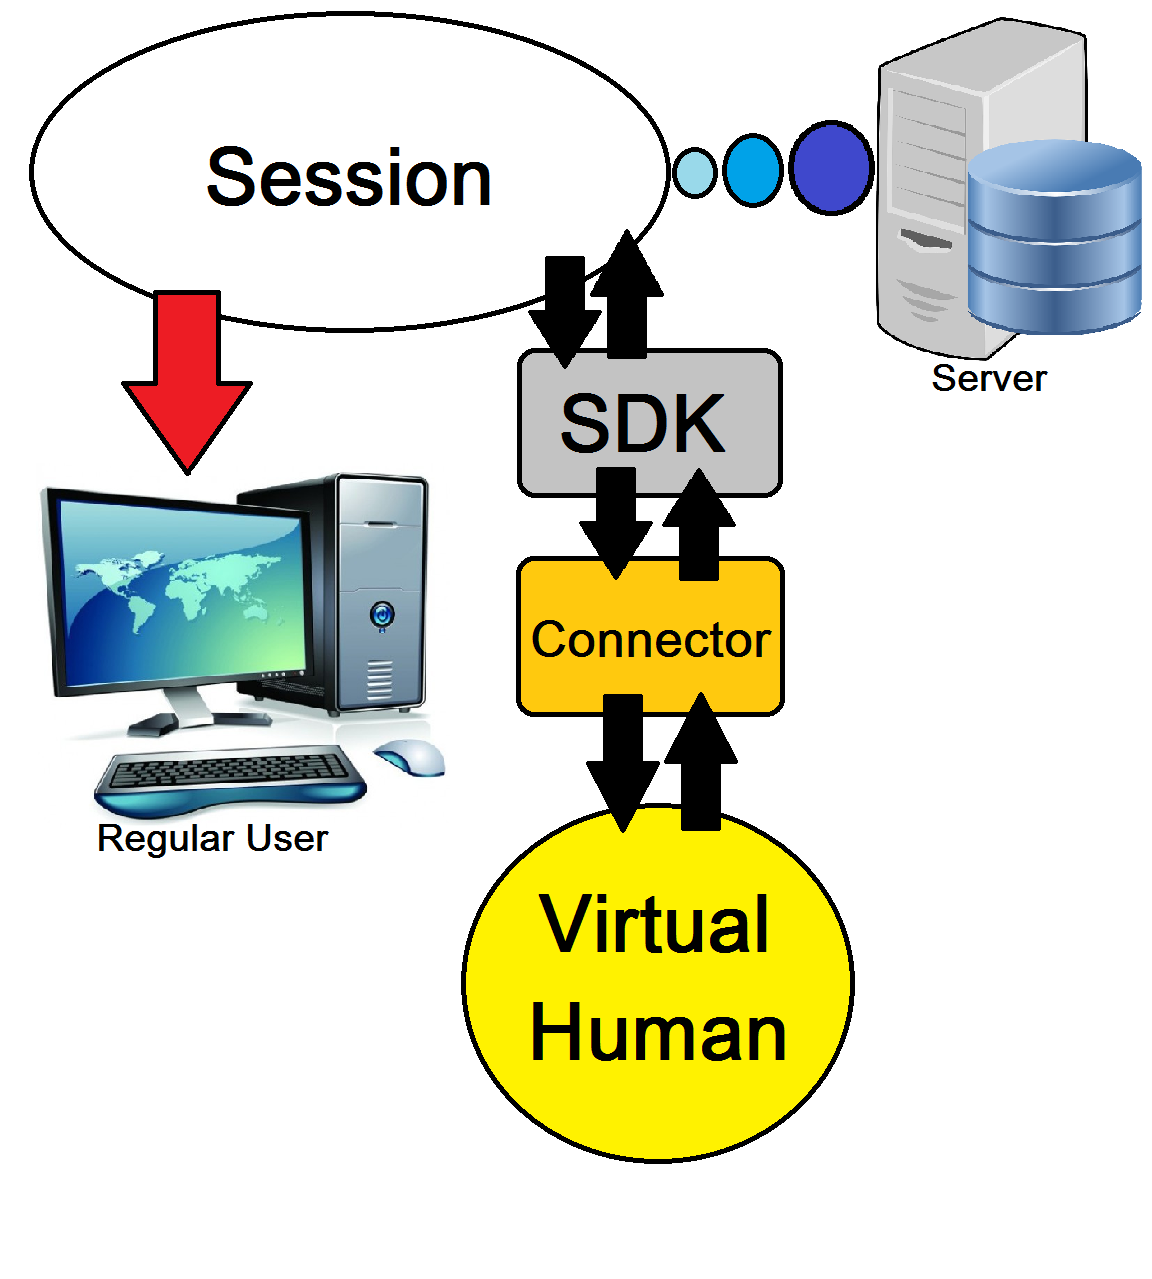
\includegraphics{Hardware_software_mapping}

\subsection{Persistent data management}
Our GOAL agent is not responsible for storing persistent data, so it does not have external files or databases. Everything is stored on the database of the Tygron server.
\subsection{Concurrency}
Our GOAL Agent is just one process. It shares recourses with other users of the tygron environment. If a deadlock occurs, this would be on the tygron environment. Our GOAL system won't have issues with deadlocks.
\newpage
